% BEÁLLÍTÁSOK - JOBB NEM VÁLTOZTATNI
\documentclass[final]{ubb_dolgozat}
\usepackage{definitions}

% pszeudokód írás végett
\usepackage{algpseudocode}
\usepackage[chapter]{algorithm}

% képek miatt
% \usepackage[justification=centering]{caption}
\usepackage{subcaption}
\captionsetup[table]{skip=10pt}
\captionsetup{subrefformat=parens}

% táblázatok
\usepackage{tabularx}
\usepackage{makecell}
\usepackage{multirow}

% listák
\usepackage[shortlabels]{enumitem}

% hasznos rövidítések
\providecommand{\abs}[1]{\lvert#1\rvert}
\DeclareMathOperator*{\argmin}{arg\,min}
\DeclareMathOperator*{\argmax}{arg\,max}

\providecommand{\keywords}[1]
{
  \small
  \textbf{\textit{Keywords:}} #1
}

% milyen nyelveken akarunk forráskódot megjeleníteni
\lstloadlanguages{Python}
% más lehetőségek:
% C, Matlab, Mathematica, Octave, Pascal, Perl, Python
% SCilab, SQL, Haskell, Lisp, Lua, make, ML, PHP, Prolog
%
% a teljes lista a LISTINGS csomagban.


% ezt be lehet tenni MINDEGYIK megjelenítendő kód elé opcióként
\lstset{language=Python}


%%%%%%%%%%%%%%%%%%%%%%%%%%%%%%%%%%%%%%%%%%%%%%%
%%!!          EZT KELL VÁLTOZTATNI       !!%%%%
%%     A DOLGOZAT CÍMOLDALÁNAK ELEMEI        %%

%% MELYIK ÉVBEN ADJUK LE
\submityear{%
2020
}

\titleHU{%
Kritikus csomópontok meghatározása komplex hálózatokban
}

% Az alábbi sorokat ki kell tölteni!

\titleEN{%
Critical node detection problem in complex networks
}

\titleRO{%
Identificarea nodurilor critice în rețele complexe
}

\author{%
Béczi Eliézer
}

%%
\tutorHU{%
dr. Gaskó Noémi,\newline egyetemi docens\\
% a hozzátartozás akkor szükséges, ha NEM BBTE-s a tanár
%{\large Babe\c{s}--Bolyai Tudományegyetem,\\
% Matematika és Informatika Kar}% ha különbözik, akkor fel kell tűntetni
}
%%
\tutorRO{%
Conf. dr. Gaskó Noémi\\
% az egyetem akkor szükséges, ha nem BBTE-s a tanár, a minta a BBTE-t
% tartalmazza
% {\large Universitatea Babe\c{s}--Bolyai,\\ % dacã diferã!!!
% Facultatea de Matematic\u{a} \c{s}i Informatic\u{a} }%
}
%%
\tutorEN{%
Assoc. prof. dr. Gaskó Noémi
% {\large Babe\c{s}--Bolyai University,\\
% Faculty of Mathematics and Informatics}
}


% 
%\includeonly{bevezet}


\begin{document}

% ez a címoldal része
\maketitle

%% ABSTRACT
\begin{abstractEN} % ANGOL VÁLTOZAT
  {
    \vfill
    The purpose of this paper is to address the critical node detection problem (CNDP).
    The CNDP is an optimization problem that consists of finding a subset of nodes that the deletion of will greatly decrease the connectivity of the network.
    We approach the problem from two different perspectives: from a single-objective and a bi-objective standpoint.
    The single-objective formulation of the CNDP aims to minimize the pairwise connectivity of the graph, whereas the goal of the bi-objective one (BOCNDP) is to maximize the number of connected components while simultaneously minimizing the variance of their cardinalities.
    For solving the CNDP we propose three different algorithms: a greedy, a genetic and a memetic algorithm.
    In the case of the BOCNDP, we use six common MOEAs (NSGA-II, PAES etc.), and experiment with different dominance operators, such as Pareto-, Nash- and Berge-dominance.
    Finally, we give a brief comparison of the algorithms using a benchmark set that contains four groups of graphs with different characteristics (Barabási–Albert, Erdős–Rényi etc.).
    \\[.5cm]
    \keywords{
      complex networks,
      critical node detection problem,
      single-objective,
      bi-objective,
      evolutionary algorithms,
      game theory
    }
    \vfill
  }
  \vspace*{.5cm}
  This work is the result of my own activity. I have neither given nor received unauthorized assistance on this work.
\end{abstractEN}

% a dolgozat tartalomjegyzéke -- ez automatikusan generálódik a STRUKTÚRA alapján.
{
\baselineskip 1ex
\parskip 1ex
\tableofcontents
}


%%%%%%%%%%%%%%%%%%%%%%%%%%%%%%%%%%%%%%%%%%%%%%%%%%%%%%%%%%%
%%%%%%%%%%         a dolgozat tartalma         %%%%%%%%%%%%

% ajánlott külön file-okba írni az egyes fejezeteket,
% ugyanis úgy jobban át lehet látni.


% a bevezető fejezet FILE-ja.
\include{bevezet}

% saját fejezetek
% !TeX root = ../../thesis.tex
%%%%%%%%%%%%%%%%%%%%%%%%%%%%%%%%%%%%%%%%%%%%%%%%%%%%%%%%%%%%%%%%%%%%%%%
\chapter{Bevezető}\label{ch:BEVEZETO}

Hálózatok terén nem minden csomópont egyforma fontosságú.
A kulcsfontosságú csomópontok keresésével hálózatokban széles körben foglalkoznak,
különösképpen olyan csomópontok esetén, melyek a hálózat konnektivitásához köthetők.
Ezeket a csomópontokat általában úgy nevezzük, hogy Kritikus Csomópontok.

Kritikus Csomópontok Meghatározásának Problémája (CNDP)
egy optimalizációs feladat, amely egy olyan csoport csomópont
megkereséséből áll, melyek törlése maximálisan rontja a hálózat
konnektivitását bizonyos predefiniált konnektivitási metrikák szerint.

A CNDP számos alkalmazási területtel rendelkezik.
Például, közösségi hálók nagy befolyással bíró egyedeinek azonosítása,
komputációs biológiában kapcsolatok definiálására jelút
vagy fehérje-fehérje kölcsönhatás hálózatokban,
smart grid sebezhetőségének azonosítása, egyének meghatározása
védőoltással való ellátásra vagy karanténba való zárásra egy
fertőzés terjedésének gátlása érdekében.

A CNDP egy $\mathcal{N}\mathcal{P}$-teljes feladat. Adva van egy $G = (V, E)$ gráf, ahol $|V| = n$ a csomópontok száma,
és $|E| = m$ pedig az élek száma. A feladat $K$ kritikus csomópont meghatározása, amelyek törlése a bemeneti
gráfból minimalizálja a hálózat páronkénti konnektivitását. Az alapján, hogy mit értünk egy hálózat
konnektivitása alatt, a CNDP-nak van egycélú illetve többcélú megfogalmazása is.

Ebben a dolgozatban többek között egy bi-objektív megfogalmazásával fogunk foglalkozni a CNDP-nak.
Hat standard evolúciós algoritmust (NSGAII, EpsMOEA, SPEA2, IBEA, PAES, EpsNSGAII) fogunk összehasonlítani
egymással különböző szintetikus bemenetekre (Barabási-Albert, Watts-Strogatz, Forest Fire és Erdős-Rényi),
illetve való világból inspirált bemenetekre, ugyanakkor célunk egy új hibrid algoritmus fejlesztése,
melynek eredményei összehasonlíthatóak a standard algoritmusok eredményeivel.

\section{Egycélú CNDP}

\section{Kétcélú CNDP}


\chapter{Egycélú CNDP}\label{ch:EGYCELU_CNDP}

\section{Páronkénti konnektivitás}\label{sec:PAIRWISE_CONNECTIVITY}
Egycélú CNDP esetén a kihívás abban áll, hogy találjunk egy olyan konnektivitási metrikát,
amely alkalmazási területtől függően megfelelően leírja egy gráf összefüggőségét.
$S$-el fogjuk jelölni a törlendő csomópontok halmazát,
míg az$f(S)$ jóság függvény fogja jellemezni a $G[V \setminus S]$ feszített részgráf összefüggőségét.
Ha $H$-val jelöljük a $G[V \setminus S]$ feszített részgráf összefüggő komponenseinek a halmazát,
akkor a jóság függvény a következő képlettel írható le:
\begin{equation}\label{eqn:PAIRWISE_CONNECTIVITY}
  f(S) = \sum_{h \in H} \frac{\abs{h} \cdot (\abs{h} - 1)}{2},
\end{equation}
amelyet az irodalom \cite{ventresca2012global, aringhieri2016general} úgy tart számon,
hogy \textbf{páronkénti konnektivitás}.
Tehát a feladat \aref{eqn:PAIRWISE_CONNECTIVITY} függvénynek a minimalizálása:
\begin{equation}\label{eqn:MIN_PAIRWISE_CONNECTIVITY}
  \min_{S \subseteq V} f(S).
\end{equation}

\Aref{eqn:PAIRWISE_CONNECTIVITY} fitnesz függvény implementációját \aref{lst:PAIRWISE-CONNECTIVITY}. kódrészlet szemlélteti Python-ban.
\lstinputlisting[
  language={Python},
  caption={Páronkénti konnektivitás},
  label={lst:PAIRWISE-CONNECTIVITY}
]{./progfiles/single-objective-cndp/pairwise_connectivity.py}


\subsubsection{Egy példa}
\Aref{fig:CNDP_EXAMPLE}. ábrán látható gráfban,
ha $k = 2$ kritikus csomópontot kell azonosítanunk,
akkor $S = \left\{ 6, 7 \right\}$ eredményezi az optimális megoldást.
A $G\left[ V \setminus S \right]$ feszített részgráf két, egyenként öt csomópontból álló összefüggő komponensre esik szét,
vagyis $\abs{H} = 2$. Így \aref{eqn:PAIRWISE_CONNECTIVITY} jóság függvény a következőképpen számolódik:
\[
  f(S) = \dfrac{5 \cdot (5 - 1)}{2} + \dfrac{5 \cdot (5 - 1)}{2} = 20.
\]

Látható, hogy nem elegendő csupán fokszám alapján csomópontokat kritikusnak nyilvánítani,
mivel az esetek túlnyomó többségében ez nem fog jó megoldáshoz vezetni.
Például, ha \aref{fig:CNDP_EXAMPLE}. ábrán található gráfban a két legnagyobb fokszámmal rendelkező nódust $S = \left\{5,9\right\}$ töröljük,
akkor a $G$ gráf ugyan szétesik $\abs{H} = 2$ komponensre,
de az eredmény jósága $f(S) = \dfrac{1 \cdot (1 - 1)}{2} + \dfrac{9 \cdot (9 - 1)}{2} = 36$ számottevően rosszabb.


\begin{figure}[t]
  \centering
  \begin{tabular}{ll}
    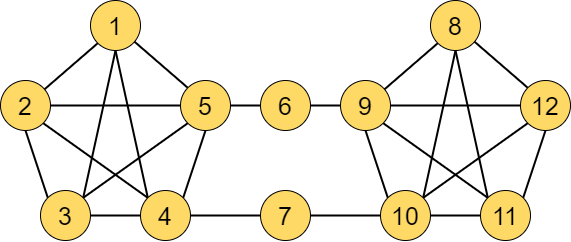
\includegraphics[scale=0.3]{images/cndp_before.png}
     &
    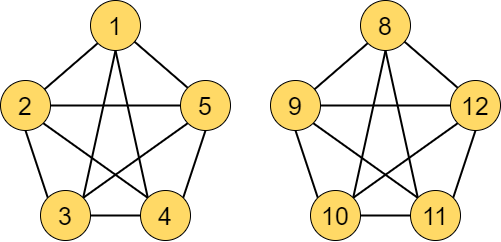
\includegraphics[scale=0.3]{images/cndp_after.png}
  \end{tabular}
  \caption{
    Példa egy kis méretű gráfra (bal oldalt), amely a 6. és 7. csomópontok törlése után
    szétesik két összefüggő komponensre (jobb oldalt).
  }
  \label{fig:CNDP_EXAMPLE}
\end{figure}


\chapter{Kétcélú CNDP}\label{ch:KETCELU_CNDP}

\section{Többcélú optimalizálás}
A gyakorlatban számos olyan optimalizálási probléma létezik, ahol nem tudunk egyetlen egyértelmű célfüggvényt meghatározni, például:
\begin{itemize}
  \item[\textbullet] egy épület megtervezésekor minimalizálni szeretnénk az energia fogyasztást és az építési költséget, de ugyanakkor maximalizálni a termikus kényelmet \cite{nguyen2014review};
  \item[\textbullet] több projekt elvállalásakor minimalizálni szeretnénk az összköltséget és a szükséges projektvezetők számát, és maximalizálni a projektek összfontosságát és a befejezett projektek számát \cite{alothaimeen2019overview};
  \item[\textbullet] egy kőolajfinomító esetén maximalizálni szeretnénk a benzin hozamot, de ugyanakkor minimalizálni a különböző kémiai reakciók során termelődő koksz mennyiségét, amely lerakódik a katalizátorra, és csökkenti ennek reaktivitását \cite{kasat2003multi}.
\end{itemize}

Tehát ezekben az esetekben nem csak egy $f$ célfüggvényünk van, hanem több darab (pl. energia fogyasztás célfüggvénye, termikus kényelem célfüggvénye, stb.), amelyek halmazát $F$-el fogjuk jelölni.
Külön-külön az egyes célfüggvények a következő indexelt formában írhatók fel:
\begin{equation}\label{eqn:OBJECTIVE_FUNCTIONS}
  f_i \colon \mathbb{P} \to \mathbb{R}, i \in \left\{ 1, 2, \dots, \abs{F} \right\},
\end{equation}
ahol $P$ az értelmezési tartomány.

\section{A CNDP-től a BOCNDP-ig}

Az egycélú CNDP-től úgy jutunk el a kétcélú CNDP-ig, hogy nem egy függvényt fogunk optimalizálni, hanem kettőt.
Míg a CNDP esetén \aref{eqn:PAIRWISE_CONNECTIVITY} képlettel leírt függvény minimalizálása volt a feladat,
addig a BOCNDP esetén két célfüggvényünk van, amelyeket optimalizálni szeretnénk $k$ csomópont kitörlése után a $G$ gráfból:
\begin{enumerate}
  \item Maximalizálni szeretnénk az összefüggő komponensek számát.
  \item Minimalizálni szeretnénk az összefüggő komponensek számosságának a varianciáját.
\end{enumerate}
Ennek érdekében a következő két célfüggvényt vezetjük be:
\begin{equation}\label{eqn:MAX_CONNECTED_COMPONENTS}
  \max \quad \abs{H},
\end{equation}
\begin{equation}\label{eqn:MIN_CARDINALITY_VARIANCE_COMPONENTS}
  \min \quad var(H),
\end{equation}
ahol $H$-val jelöljük a $G\left[ V \setminus S \right]$ feszített részgráf összefüggő komponenseinek a halmazát,
és $var(H)$ jelöli az összefüggő komponensek számosságának nem szabályos mintavételének a varianciáját.
A H halmaz varianciáját a következő képlet segítségével számoljuk ki:
\begin{equation}\label{eqn:CARDINALITY_VARIANCE_COMPONENTS}
  \dfrac{1}{ \abs{H} } \sum_{h \in H} \left( \abs{h} - \dfrac{ n^{*} }{ \abs{H} } \right)^{2},
\end{equation}
ahol $n^{*} = \sum_{h \in H} \abs{h}$ a $G\left[ V \setminus S \right]$ feszített részgráf csomópontjainak a száma.

\Aref{eqn:MAX_CONNECTED_COMPONENTS} és \aref{eqn:CARDINALITY_VARIANCE_COMPONENTS}
képletekkel leírt problémát úgy ismerjük az irodalomban \cite{ventresca2018bi}, mint \textbf{BOCNDP}.
A CNDP is ugyanerre a problémára nyújt megoldást azáltal,
hogy ezt a két függvényt egyesíti \aref{eqn:PAIRWISE_CONNECTIVITY} függvényben,
melynek minimalizálása (lásd \aref{eqn:MIN_PAIRWISE_CONNECTIVITY} egyenlet) maximalizálni fogja a komponensek számát, amelyekre szétesik az eredeti gráf,
de ugyanakkor minimalizálja is a komponensek közötti varianciát.

A $H$ halmaz számosságának meghatározását \aref{lst:NO-CONNECTED-COMPONENTS}. kódrészlet mutatja be Python-ban,
míg \aref{eqn:CARDINALITY_VARIANCE_COMPONENTS} képlet implementációját \aref{lst:CARDINALITY-VARIANCE-COMPONENTS}. kódrészlet.


\begin{figure}[h]
  \centering
  \begin{tabular}{ll}
    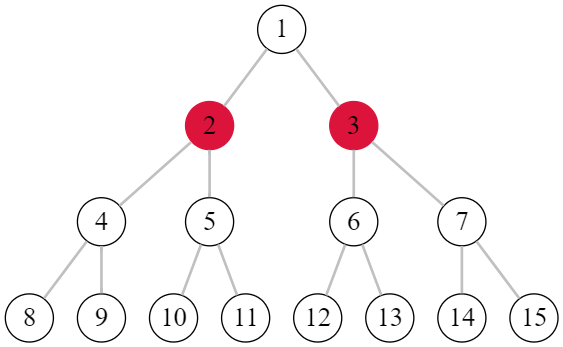
\includegraphics[scale=0.4]{images/bocndp_before.png}
     &
    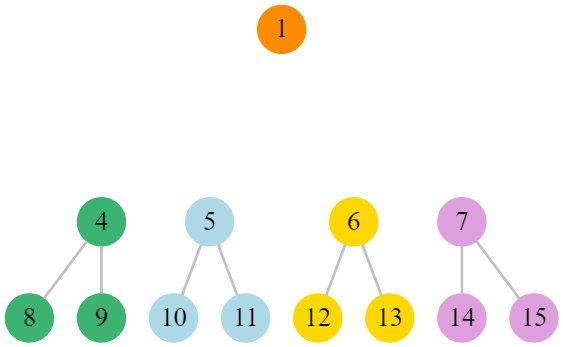
\includegraphics[scale=0.4]{images/bocndp_after.png}
  \end{tabular}
  \caption{
    Példa egy kis méretű gráfra (bal oldalt), amely a 2. és 3. csomópontok (piros színnel emeltük ki ezeket) törlése után
    szétesik öt összefüggő komponensre (jobb oldalt), amelyeket különböző színekkel jelöltünk meg a könnyebb láthatóság kedvéért.
  }
  \label{fig:BOCNDP_EXAMPLE}
\end{figure}

\subsubsection{Egy példa}
\Aref{fig:BOCNDP_EXAMPLE} ábrán látható gráfban, ha $k = 2$ kritikus csomópontot kell azonosítanunk,
akkor $S = \left\{ 2, 3 \right\}$ eredményezi az optimális megoldást.
A $G\left[ V \setminus S \right]$ feszített részgráf szétesik egy egy csomópontból álló,
és négy három csomópontból álló komponensre, vagyis $\abs{H} = 5$.
Így \aref{eqn:CARDINALITY_VARIANCE_COMPONENTS} képlettel leírt komponensek közötti variancia a következőképpen számolható ki:
\[
  var(H) = \dfrac{1}{5} \cdot \left[ \left( 1 - \dfrac{13}{5} \right)^{2} + 4 \cdot \left( 3 - \dfrac{13}{5} \right)^{2} \right] = \dfrac{16}{25} = 0.64.
\]


\lstinputlisting[
  language={Python},
  caption={A feszített részgráf összefüggő komponenseinek a száma},
  label={lst:NO-CONNECTED-COMPONENTS}
]{./progfiles/bi-objective-cndp/no_connected_components.py}

\lstinputlisting[
  language={Python},
  caption={Az összefüggő komponensek számosságának a varianciája},
  label={lst:CARDINALITY-VARIANCE-COMPONENTS}
]{progfiles/bi-objective-cndp/cardinality_variance_components.py}

\section{Kísérleti előkészítés}\label{sec:KISERLETI_ELOKESZITES}

Ebben a részben bemutatjuk a BOCNDP probléma megoldására javasolt genetikus algoritmusokat és ezek paraméterezéseit.
Az algoritmusok a \emph{Platypus keretrendszerben} \cite{hadka2017platypus} találhatóak, a keretrendszer által biztosított osztályokat fogjuk használni.

\begin{description}
      \itemsep-0.5em
      \item[NSGAII] -- Az NSGAII (Non-dominated Sorting Genetic Algorithm II) \cite{deb2002fast} az egyik legnépszerűbb többcélú optimalizáló algoritmus,
            amely az NSGA továbbfejlesztett változata. Az NSGAII a megszokott rekombinációs és mutációs genetikai operátorokon kívül,
            amelyek új egyedek létrehozásáért felelősek, két másik különleges mechanizmust használ a következő generáció populációjának létrehozásához:
            \textit{nem-dominált rendezés}\footnote{ Angolul: non-dominated sorting. } révén a populációt alpopulációkra
            osztja valamilyen dominancia által meghatározott sorrend alapján (pl. Pareto, Nash vagy Berge dominancia),
            és kiszámítja az alpopulációk egyedei közötti \textit{tömörülési távolságot}\footnote{ Angolul: crowding distance. },
            felállítva egy sorrendet az alpopulációk egyedei között, hogy az elszigetelt megoldásokat részesítse előnyben.
            % \item[~]
      \item[EpsMOEA] -- Az EpsMOEA (Epsilon Multi-Objective Evolutionary Algorithm) \cite{deb2003towards} egy egyensúlyi állapotú evolúciós algoritmus,
            amely $\epsilon$-dominancia archiválást használ a populáció sokszínűségének fenntartása végett.
      \item[SPEA2] -- A SPEA2 (Strength Pareto Evolutionary Algorithm 2) \cite{zitzler2001spea2} feladata, hogy megtaláljon és fenntartson egy frontnyi nem-dominált megoldást,
            ideális esetben egy halmaznyi Pareto-optimális megoldást. Ennek elérése érdekében egy evolúciós eljárást használ
            - felhasználva a genetikai rekombinációs és mutációs operátorokat - a megoldástér felderítése végett,
            és egy szelekciós eljárást, amely fitnesz függvénye egy egyed domináltságának és a becsült Pareto-front zsúfoltságának a kombinációja.
            A nem-dominált megoldások halmazáról egy archívum van karbantartva, amely különbözik az evolúciós eljárásban használt megoldások populációjától,
            biztosítva ezáltal egy elitista kiválasztást.
      \item[IBEA] -- Az IBEA (Indicator Based Evolutionary Algorithm) \cite{zitzler2004indicator} alapötlete, hogy egy \textit{bináris hipertérfogat indikátort} használ a szelekciós eljárás szakaszában,
            amikor elválik, hogy mely egyedek fognak tovább élni, a következő generáció alapjául szolgálva.
      \item[PAES] -- A PAES (Pareto Archived Evolution Strategy) \cite{knowles1999pareto} egy többcélú optimalizáló, amely két fő céllal lett kifejlesztve.
            Az elsődleges cél, hogy szigorúan lokális keresésre korlátozódik: a jelenlegi megoldást csak kis mértékben változtatja (mutáció),
            ezáltal eljutva a jelenlegi megoldástól egy szomszédos megoldásig. Ez a folyamat jelentős mértékben megkülönbözteti más többcélú optimalizáló genetikus algoritmustól (pl. NSGAII, SPEA2, IBEA),
            amelyek egy populációnyi megoldással dolgoznak, és ezen egyedek segítségével történik meg a keresztezés és kiválasztás.
            A második cél, hogy az algoritmus egy valódi Pareto optimalizáló kell, hogy legyen, minden nem-dominált megoldást egyformán kezelve.
            Mindkét cél elérése azonban elég problémás, mert az esetek többségében, amikor egy pár megoldást összehasonlítunk, akkor egyik sem fogja dominálni a másikat.
            A PAES ezt úgy oldja meg, hogy karbantart egy archívumot a nem-dominált megoldások halmazáról, amely révén felbecsüli az új megoldás jóságát.
      \item[EpsNSGAII] -- Az EpsNSGAII (Epsilon NSGAII) \cite{kollat2005value} az NSGAII egy kibővített változata, amely $\epsilon$-dominancia archiválást használ.
            Továbbá, véletlenszerű újraindítás jellemzi, biztosítva ezáltal egy változatosabb megoldáshalmazt.
\end{description}

Mindegyik algoritmus esetén a Platypus keretrendszer által felkínált alapértelmezett paramétereket használjuk:
$N = 100$ a populáció mérete;
$k = 2$ nagyságú versengő kiválasztás;
SSX keresztezés;
$\epsilon = 0.05$;
$c = 100$ az archívum kapacitása, és $b = 8$ a kettéosztások száma;
$t_{\max} = 10\,000$ az iterációszám.

\section{Dominancia operátorok}
A multikritériumú genetikus algoritmusok esetén felmerül a kérdés, hogy miként döntjük el, hogy egy megoldás jobb-e vagy rosszabb, mint egy másik.
Viszont az is megtörténhet, hogy két megoldás összehasonlíthatatlan.
Ennek a kérdésnek a megválaszolása érdekében szükséges bevezetnünk a \emph{dominancia operátor} fogalmát.
A dominancia operátor fontos szerepet lát el a multikritériumú genetikus algoritmusok keretein belül,
mivel a \emph{dominancia reláció} segítségével lesz eldöntve, hogy két megoldás közül melyik dominálja melyiket, vagy hogy egyik sem dominálja a másikat.bemutatott multikritériumú genetikus algoritmusok mindegyike esetén több típusú dominanciát fogunk kipróbálni kísérleti célokból.
Ezeket a dominancia típusokat szeretnénk a következőkben ismertetni.


\subsection{Pareto-dominancia}
\begin{ert}
  Azt mondjuk, hogy egy $x$ megoldás \emph{Pareto-dominál} egy $y$ megoldást $\left( x \prec y \right)$, ha teljesül a következő két feltétel:
  \begin{align*}
    \forall i \in \left\{ 1, 2, \dots, \abs{F} \right\} \colon f_i(x) \leq f_i(y), \\
    \exists j \in \left\{ 1, 2, \dots, \abs{F} \right\} \colon f_j(x) < f_j(y).
  \end{align*}

  Tehát az $x$ megoldás minden szempontból legalább olyan jó, mint az $y$, és legalább egy szempontból még jobb is nála.
\end{ert}


% \subsubsection{Pareto-optimum}
\begin{ert}
  A Pareto-dominancia segítségével bevezethetjük az optimum fogalmát.
  Egy $\hat{x}$ \emph{Pareto-optimum}, ha nincs még egy olyan megoldásjelölt, ami dominálná őt:
  \[
    \nexists x \in \mathbb{P} \colon x \prec \hat{x}.
  \]
\end{ert}


% \subsubsection{Pareto-front}
\begin{ert}
  Gyakran megtörténik, hogy nem csak egy, hanem több Pareto-optimális megoldásunk van.
  Ebben az esetben a Pareto-optimális megoldások halmazát nevezzük \emph{Pareto-frontnak}.
\end{ert}


% \subsubsection{Egy példa}
\begin{pld}
  \Aref{fig:PARETO_DOMINANCE}. ábra egy példát mutat a Pareto-optimumokra.
  A probléma két célfüggvény optimalizálásából tevődik össze: az $f_1$ célfüggvény maximalizálásából és az $f_2$ célfüggvény minimalizálásából.
  Tehát egy pont minél távolabb van az origótól az X-tengelyen, de ugyanakkor minél közelebb hozzá az Y-tengelyen, annál jobb.

  Néhány következtetés, ami leolvasható a diagramról:
  \begin{itemize}
    \item[\textbullet] $A \prec B$, mivel mindkét szempont szerint jobb nála;
    \item[\textbullet] $E \prec A$, mivel $f_2$ szempontjából azonosak, de $f_1$ szerint jobb;
    \item[\textbullet] $A \nprec D$, mert bár $f_2$ szerint jobb, de $f_1$ szempontjából rosszabb;
    \item[\textbullet] $D \nprec A$, mert bár $f_1$ szerint jobb, de $f_2$ szempontjából rosszabb;
    \item[\textbullet] $C$, $E$ pontokat senki se dominálja (ők se egymást), ezért ők alkotják a Pareto-frontot.
  \end{itemize}

  Jól látható, hogy a feladatnak nincs egyértelmű megoldása.
  A $C$ és $E$ pontok nem azonosak, mégsem tudjuk az egyiket előnyben részesíteni a másikhoz képest.
  A feladat megoldása tehát ez a két pont.
\end{pld}

\begin{meg}
  Fontos megemlítenünk, hogy ez nem hátrány, hanem éppenhogy előny.
  A Pareto-dominancia lehetővé teszi, hogy ne csak egy megoldást kapjunk vissza, hanem akár mindet.
  A többcélú feladatok megoldásánál éppen azt szeretnénk, hogy minél több nem-dominált eredményt kapjunk.
  Mivel legtöbbször a front mérete nagyon nagy, és az összes megoldást nem várhatjuk el, akkor az egymástól minél távolibbakat szeretnénk megkapni.

  Az, hogy utána melyik megoldás lesz kiválasztva, az már a felhasználó egyéni döntése.
\end{meg}

\begin{figure}[t]
  \centering
  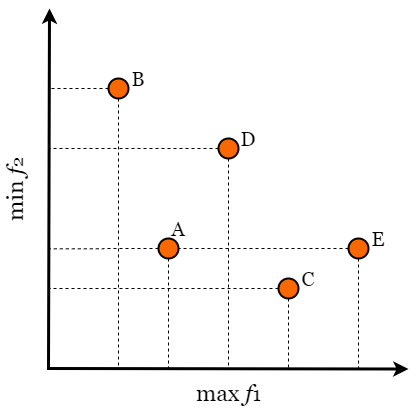
\includegraphics[scale=0.5]{images/pareto_dominance.png}
  \caption{
    Példa egy kétcélú optimalizálási feladatra, ahol az $f_1$ célfüggvényt maximalizálni, míg az $f_2$ célfüggvényt minimalizálni kell.
  }
  \label{fig:PARETO_DOMINANCE}
\end{figure}


\subsection{Nash-dominancia}
A Nash-dominancia fogalmát \citeN{lung2008computing} vezették be, és a Nash-egyensúly fogalmán alapszik.
Megértéséhez szükséges néhány, a \emph{játékelméletből} \cite{von2007theory} ismert fogalom bevezetése.


\subsubsection{Nem-kooperatív játékok}
Legyen $n > 1$ természetes szám a játékosok száma, és $I = \left\{ 1, \dots, n \right\}$ a játékosok halmaza.
Minden $i \in I$ esetén, $S_i$ az $i$-edik játékos stratégiáinak a halmaza, míg $s_i \in S_i$ a játékos tetszőleges stratégiája.
Legyen $S = S_1 \times S_2 \times \dotsc \times S_n$ a stratégiaprofilok halmaza, $s \in S$ pedig egy általános stratégiaprofil.
Minden $i \in I$ esetén, $u_i \colon S \to \mathbb{R}$ az $i$-edik játékos kifizetőfüggvénye.
Legyen $U = \left\{ u_1, \dots, u_n \right\}$ a kifizetőfüggvények halmaza.
Jelölje $\left( t_i, s_{-i} \right)$ az $\left( s_1, \dots, s_{i-1}, t_i, s_{i+1}, \dots, s_n \right)$ stratégiaprofilt,
amelyet úgy kapunk, hogy az $s$ stratégiaprofil $i$-edik játékosának a stratégiáját kicseréljük $t_i$-re, $t_i \in S_i$.


\subsubsection{Nash-egyensúly}
Az előbb bevezetett jelölések segítségével bevezethetjük a nem-kooperatív játékelmélet központi fogalmát, a \emph{Nash-egyensúlyt} \cite{nash1951non}.

\begin{ert}
  Azt mondjuk, hogy az $s^* \in S$ stratégiaprofil Nash-egyensúlyt alkot,
  ha egyik játékosnak sem érdemes egyoldalúan eltérnie a stratégiaprofilban szereplő saját stratégiájától.
  Tehát minden $i \in I$ játékos és $s_i \in S_i$ stratégia esetén, a következő egyenlőtlenség teljesül:
  \[
    u_i\left(s^*\right) \ge u_i\left(t_i, s_{-i}^*\right).
  \]
\end{ert}


\subsubsection{Nash-dominancia}
Legyen $x$ és $y$ két stratégiaprofil $S$-ből.
Bevezetünk egy $k \colon S \times S \to \mathbb{N}$ operátort, amely az $\left( x, y \right)$ pároshoz hozzárendeli a következő halmaz számosságát:
\[
  \left\{ i \in I \mid u_i(y_i, x_i) \ge u_i(x), y_i \neq x_i \right\}.
\]

A halmaz azon $i$ játékosokat tartalmazza, akik adott x stratégiaprofil esetén, hasznot húznának abból, ha megváltoztatnák stratégiájukat $x_i$-ről $y_i$-re.

\begin{ert}
  Azt mondjuk, hogy egy $x$ stratégiaprofil \emph{Nash-dominál} egy $y$ stratégiaprofilt ($x \prec y$), ha teljesül az alábbi feltétel:
  \[
    k(x,y) < k(y, x).
  \]

  Tehát egy $x$ stratégiaprofil akkor Nash-dominál egy $y$ stratégiaprofilt, ha kevesebb játékos tudja megnövelni nyereségét úgy, hogy megváltoztatja stratégiáját $x_i$-ről $y_i$-re, mint fordítva.
  Azt is mondhatjuk, hogy az $x$ stratégiaprofil stabilabb (közelebb van az egyensúlyhoz), mint az $y$ stratégiaprofil.
\end{ert}


% \subsubsection{Nash-optimum}
\begin{ert}
  A Nash-dominancia segítségével bevezethetjük az optimum fogalmát.
  Egy $s^* \in S$ stratégiaprofil \emph{Nash-optimum}, ha nincs még egy olyan stratégiaprofil, ami dominálná őt:
  \[
    \nexists s \in S, s \neq s^* \colon s \prec s^*.
  \]
\end{ert}


% \subsubsection{Nash-front}
\begin{ert}
  Gyakran megtörténik, hogy nem csak egy, hanem több Nash-optimális megoldásunk van.
  Ebben az esetben a Nash-optimális megoldások halmazát nevezzük \emph{Nash-frontnak}.
\end{ert}


% \subsubsection{Nash és a BOCNDP}
\begin{tet}\label{thm:NE_EGYENLO_NF}
  \citeN{lung2008computing} egy fontos következtetésre jutottak, miszerint minden Nash-egyensúlyt alkotó stratégiaprofil egyben Nash-optimum is, és minden Nash-optimum egyben Nash-egyensúlyt alkotó stratégiaprofil is.
\end{tet}

Ez azért rendkívül fontos eredmény, mivel lehetővé teszi számunkra, hogy evolúciós kereső operátorok (keresztezés, mutáció, kiválasztás) segítségével megkeressük a Nash-egyensúlyt alkotó megoldásokat.


% \subsubsection{Egy példa}
\begin{pld}
  A következőkben egy példán keresztül szeretnénk szemléltetni a Nash-dominancia és a Nash-egyensúly közötti kapcsolatot.
  \Aref{fig:NASH_DOMINANCE}. ábrán látható gráfban $k = 1$ kritikus csomópontot szeretnénk beazonosítani.
  \Aref{eqn:PAIRWISE_CONNECTIVITY} képlettel leírt függvényt fogjuk használni, mint célfüggvény vagy kifizetőfüggvény.
  Ez fogja megmondani, hogy egy megoldás vagy stratégiaprofil mennyire jó.
  Célunk a függvény minimalizálása \ref{eqn:MIN_PAIRWISE_CONNECTIVITY}, mivel minél kisebb értéket ad vissza, annál jobb az illető megoldás.

  A feladatot felfoghatjuk ugyanakkor, mint egy kétszemélyes stratégiai játék.
  \Aref{tab:NASH_DOMINANCE}. táblázat szemlélteti a feladat lemodellezett változatát, mint kétszemélyes stratégia játék:
  $I = \left\{ 1, 2 \right\}$ a játékosok halmaza, $S_1 = S_2 = \left\{ A, B, C \right\}$ a stratégiahalmazok, a kifizetéseket a mátrix tartalmazza.

  A Nash-egyensúly megtalálása érdekében mindegyik stratégiaprofilt sorra meg kell vizsgáljuk.
  Ne felejtsük, hogy minél kisebb a szám, annál nagyobb a játékos nyeresége.
  \begin{itemize}
    \item[$(A, A)$] -- A $C$ stratégiát választva az $A$ helyett, az első játékos előnyhöz jut, hiszen $u_1(C, A) = 0 < 1 = u_1(A, A)$.
          Ezért ez a stratégiaprofil nem alkot Nash-egyensúlyt.
          Továbbá a második játékos is megnövelheti nyereségét, ha $A$ helyett $C$-t választ, mivel $u_2(A, C) = 0 < 1 = u_2(A, A)$.
    \item[$(A, B)$] -- Ugyanaz a helyzet, mint az $(A, A)$ stratégiaprofil esetén, ezért nem alkot Nash-egyensúlyt.
    \item[$(A, C)$] -- A $C$ stratégiát választva az $A$ helyett, az első játékos előnyhöz jut, hiszen $u_1(C, A) = 0 < 1 = u_1(A, A)$.
          Ezért ez a stratégiaprofil nem alkot Nash-egyensúlyt.
    \item[$(B, A)$] -- Ugyanaz a helyzet, mint az $(A, A)$ stratégiaprofil esetén, ezért nem alkot Nash-egyensúlyt.
    \item[$(B, B)$] -- Ugyanaz a helyzet, mint az $(A, A)$ stratégiaprofil esetén, ezért nem alkot Nash-egyensúlyt.
    \item[$(B, C)$] -- Ugyanaz a helyzet, mint az $(A, C)$ stratégiaprofil esetén, ezért nem alkot Nash-egyensúlyt.
    \item[$(C, A)$] -- A $C$ stratégiát választva az $A$ helyett, a második játékos előnyhöz jut, hiszen $u_2(C, C) = 0 < 1 = u_2(C, A)$.
          Ezért ez a stratégiaprofil nem alkot Nash-egyensúlyt.
    \item[$(C, B)$] -- Ugyanaz a helyzet, mint a $(C, A)$ stratégiaprofil esetén, ezért nem alkot Nash-egyensúlyt.
    \item[$(C, C)$] -- Egyik játékos sem tudja megnövelni nyereségét úgy, hogy a jelenlegi stratégiája helyett egy másikat választ.
          Ezért ez a stratégiaprofil Nash-egyensúlyt alkot.
  \end{itemize}

  Következtetésként elmondhatjuk, hogy ennek a játéknak egy Nash-egyensúlya van, ami nem más, mint a $(C, C)$ stratégiaprofil.

  Ha \aref{sec:KISERLETI_ELOKESZITES} részben bemutatott bármelyik multikritériumú genetikus algoritmus esetén lecseréljük az általa használt Pareto-dominanciát Nash-dominanciára,
  akkor az algoritmus által meghatározott Nash-front egyetlen Nash-optimális megoldásból fog állni, ami nem lesz más, mint az $S = \left\{ C, C \right\}$ halmaz.

  Láthatjuk, hogy \aref{thm:NE_EGYENLO_NF} tétel igaz, vagyis használhatjuk a multikritériumú genetikus algoritmusokat Nash-egyensúly egyensúlypont-keresésre.
\end{pld}

\begin{figure}[t]
  \begin{minipage}{\textwidth}
    \begin{minipage}[b]{0.3\textwidth}
      \centering
      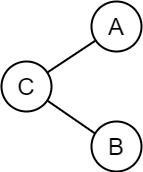
\includegraphics[scale=0.5]{images/nash_dominance.png}
      \vspace*{2.5mm}
      \captionof{figure}{Példa egy három csomópontból álló útgráfra.}
      \label{fig:NASH_DOMINANCE}
    \end{minipage}
    \hfill
    \begin{minipage}[b]{0.65\textwidth}
      \centering
      \resizebox{0.8\textwidth}{!}{
        \begin{tabular}{ccccc}
                                                             &                                 & \multicolumn{2}{c}{Második játékos} &                                                                   \\ \cline{2-5}
          \multicolumn{1}{c|}{}                              & \multicolumn{1}{c|}{}           & \multicolumn{1}{c|}{\textit{A}}     & \multicolumn{1}{c|}{\textit{B}} & \multicolumn{1}{c|}{\textit{C}} \\ \cline{2-5}
          \multicolumn{1}{c|}{\multirow{2}{*}{Első játékos}} & \multicolumn{1}{c|}{\textit{A}} & \multicolumn{1}{c|}{$1; 1$}         & \multicolumn{1}{c|}{$1; 1$}     & \multicolumn{1}{c|}{$1; 0$}     \\ \cline{2-5}
          \multicolumn{1}{c|}{}                              & \multicolumn{1}{c|}{\textit{B}} & \multicolumn{1}{c|}{$1; 1$}         & \multicolumn{1}{c|}{$1; 1$}     & \multicolumn{1}{c|}{$1; 0$}     \\ \cline{2-5}
          \multicolumn{1}{c|}{}                              & \multicolumn{1}{c|}{\textit{C}} & \multicolumn{1}{c|}{$0; 1$}         & \multicolumn{1}{c|}{$0; 1$}     & \multicolumn{1}{c|}{$0; 0$}     \\ \cline{2-5}
        \end{tabular}
      }
      \captionof{table}{A bal oldalon található gráf leképezése egy kétszemélyes stratégiai játékra.}
      \label{tab:NASH_DOMINANCE}
    \end{minipage}
  \end{minipage}
\end{figure}


\subsection{Berge-dominancia}


\section{A Platypus keretrendszer}\label{sec:PLATYPUS_FRAMEWORK}


A Platypus keretrendszert \citeN{hadka2017platypus} fejlesztette ki.
Ez egy evolúciós számítások elvégzésére szolgáló keretrendszer, amely a többcélú evolúciós algoritmusokra összpontosít.
A keretrendszer a következő elemekből tevődik össze:

\begin{itemize}
  \itemsep-0.17em
  \item[\textbullet] többcélú evolúciós algoritmusokból (NSGAII, NSGAIII, EpsMOEA stb.);
  \item[\textbullet] szelekciós operátorokból (versengő kiválasztás);
  \item[\textbullet] rekombinációs operátorokból (SBX, PCX, HUX stb.);
  \item[\textbullet] mutációs operátorokból (PM, UM, BM stb.);
  \item[\textbullet] reprezentációk különböző típusaiból (valós, bináris, részhalmaz stb.);
  \item[\textbullet] dominancia operátorokból (Pareto-dominancia, $\epsilon$-dominancia, attribútum-dominancia).
\end{itemize}

A Platypus keretrendszer modularizáltságának köszönhetően könnyű új algoritmusokkal vagy operátorokkal kibővíteni a rendszert.
De nem csak kibővíteni lehet, hanem meglévő algoritmusok által használt elemeket lecserélni már meglévő vagy általunk definiált elemekre.
Így az algoritmus váza nem változik, viszont lehetőség nyílik különböző operátorok összehasonlítására egy algoritmus esetén.

A következőkben \aref{sec:DOMINANCIA_OPERATOROK}. részben bemutatott dominancia operátorok implementációt szeretnénk ismertetni a Platypus keretrendszer által biztosított környezetben.

% Nash
\subsection{Operátorok definiálása}


\subsubsection{Nash-dominancia}
\Aref{lst:BOCNDP-NASH-DOMINANCE}. kódrészlet szemlélteti \aref{eqn:NASH_DOMINANCIA} képlettel leírt Nash-dominancia implementációját a Platypus keretrendszer segítségével.

\lstinputlisting[
  language={Python},
  caption={A Nash-dominancia implementációja a Platypus keretrendszerben.},
  label={lst:BOCNDP-NASH-DOMINANCE}
]{./progfiles/bi-objective-cndp/bocndp_nash_dominance.py}

Ahhoz, hogy egy új dominancia operátort vezethessünk be a rendszerbe, amit majd kipróbálhatunk különböző multikritériumú genetikus algoritmusok esetén,
egy osztályt kell létrehoznunk, amely a Platypus keretrendszer által biztosított \emph{Dominance} osztályt örököli.
Ezt az osztályt mi úgy neveztük el, hogy \emph{NashDominance}, és a \emph{Dominance} szülőosztály egyetlen metódusát írja fölül, a \emph{compare} metódust.

A \emph{compare} eljárás fog két megoldást - $x$ és $y$ - összehasonlítani, és visszatéríti, hogy melyik Nash-dominálja melyiket, vagy hogy egyik sem dominálja a másikat.
A metódus \aref{lst:NO-CONNECTED-COMPONENTS}. és \aref{lst:CARDINALITY-VARIANCE-COMPONENTS}. kódrészletekkel szemléltetett függvényeket használja:
az első a gráf összefüggő komponenseit számolja ki, a második pedig az összefüggő komponensek számosságának a varianciáját (lásd \aref{eqn:CARDINALITY_VARIANCE_COMPONENTS} egyenletet).
Ezeket a célfüggvényeket akarjuk optimalizálni: az elsőt maximalizálni, míg a másodikat minimalizálni.


\subsubsection{Berge-dominancia}
\Aref{lst:BOCNDP-BERGE-DOMINANCE}. kódrészlet szemlélteti \aref{eqn:BERGE_DOMINANCIA} képlettel leírt Berge-dominancia implementációját a Platypus keretrendszer segítségével.
Az operátor bevezetéséhez a rendszerbe ugyanazon lépéseket kell végrehajtanunk, mint a Nash-dominancia esetén.

\lstinputlisting[
  language={Python},
  caption={A Berge-dominancia implementációja a Platypus keretrendszerben.},
  label={lst:BOCNDP-BERGE-DOMINANCE}
]{./progfiles/bi-objective-cndp/bocndp_berge_dominance.py}


\subsection{Problémák definiálása}
Ahhoz, hogy egy bármilyen problémát meg tudhassunk oldani a Platypus keretrendszer által biztosított algoritmusokkal, szükséges először definiálnunk a feladatot.
Ebben nyújt nekünk segítséget a Platypus \emph{Problem} osztálya, amely két paramétert vár el tőlünk: a döntési változók és a célok számát.
Meg kell adjuk minden döntési változó típusát vagy reprezentációját, valamint minden cél optimalizálási irányát (minimalizálás vagy maximalizálás).
Továbbá felül kell írjuk a \emph{Problem} szülőosztály \emph{evaluate} függvényét, amely egy megoldás kiértékeléséért felelős.
A BOCNDP definiálását hívatott szemléltetni \aref{lst:BOCNDP-PROBLEM}. kódrészlet.

\lstinputlisting[
  language={Python},
  caption={A BOCNDP definiálása a Platypus keretrendszerben.},
  label={lst:BOCNDP-PROBLEM}
]{./progfiles/bi-objective-cndp/bocndp_problem.py}

Amint látható, létrehozunk egy \emph{BOCNDP} nevű osztályt, amely a Platypus által biztosított \emph{Problem} osztály leszármazottja.
A konstruktorban meghívjuk a szülőosztály \emph{init} metódusát, amely beállítja a döntési változók számát $1$-re, a célok számát pedig $2$-re.
Megmondjuk, hogy a döntési változót a $G$ gráf csomóponthalmazának egy $k$ elemű részhalmazával fogjuk ábrázolni, valamint azt, hogy az első célfüggvényt maximalizálni, míg a másodikat minimalizálni szeretnénk.

Ezután felülírjuk a \emph{Problem} osztály \emph{evaluate} metódusát. Itt történik egy megoldás tényleges kiértékelése.
Beállítjuk mint első célfüggvény \aref{lst:NO-CONNECTED-COMPONENTS}. kódrészlettel leírt függvényt, ami a $G$ gráf összefüggő komponenseinek a számát téríti,
\aref{lst:CARDINALITY-VARIANCE-COMPONENTS}. kódrészlettel leírt függvényt pedig, ami az összefüggő komponensek számosságának a varianciáját téríti, mint második célfüggvény.
Ahogy az imént említettük, az első célfüggvényt maximalizálni, míg a másodikat minimalizálni fogjuk.


\subsection{Algoritmusok definiálása}
A Platypus keretrendszer számos kész multikritériumú genetikus algoritmust tartalmaz, de lehetőséget ad új algoritmusok definiálására is az \emph{Algorithm} osztály kiterjesztése révén.
Ugyanakkor lehetővé teszi a már meglévő algoritmusok testreszabását: egy algoritmus példányosításakor vagy felépítésekor megadhatjuk argumentumként a használni kívánt operátorokat.

\lstinputlisting[
  language={Python},
  caption={A BOCNDP megoldása az NSGAII algoritmus és a Nash-dominancia használatával.},
  label={lst:BOCNDP-EXAMPLE}
]{./progfiles/bi-objective-cndp/bocndp_example.py}

\Aref{lst:BOCNDP-EXAMPLE}. kódrészlet szemlélteti az NSGAII algoritmus egy testreszabott változatának a létrehozási folyamatát,
ahol beállítjuk, hogy \aref{lst:BOCNDP-PROBLEM}. kódrészlettel leírt \emph{BOCNDP} problémát oldja meg, és \aref{lst:BOCNDP-NASH-DOMINANCE}. kódrészlettel leírt \emph{NashDominance} osztályt használja mint dominancia operátor.
Ezután lefuttatjuk az algoritmust $10\,000$-es iterációszámmal, utána pedig kiíratjuk a Nash-optimális megoldásokat.

\section{A kezdeti populáció inicializálása}


Ugyanúgy, mint \aref{ch:EGYCELU_CNDP}. fejezetben bemutatott CNDP esetén, ahol \aref{sec:MEMETIKUS_ALGORITMUS}. részben leírt memetikus algoritmus keretein belül a populációt intelligens módon inicializáltuk, a BOCNDP esetén is kísérletezni fogunk különböző inicializálási módszerekkel.
Ez azért lényeges, mert ha eleve olyan megoldásokból indulunk ki, amelyek magukban tárolnak valamit a hálózat szerkezetéről, akkor megtörténhet, hogy jobb eredményekhez jutunk rövidebb idő alatt.
Ezeket a módszereket szeretnénk a következőkben ismertetni.


\subsection{DFS alapján}
Az első módszer abban áll, hogy kiindítunk egy mélységi bejárást (DFS) a $G$ gráf egy véletlen csomópontjából,
majd az így kapott csomóponthalmaz minden $x$-edik elemét különválasztjuk, $x = \dfrac{\abs{V}}{k}$.
A különválasztott csomópontok halmaza fogja alkotni a kezdeti populáció egy egyedét.
\Aref{alg:DFS-SMART-INIT} algoritmus szemlélteti a mélységi bejáráson alapuló intelligens inicializálási módszert.
\begin{algorithm}[h]
  \caption{Depth-first search solution generator}\label{alg:DFS-SMART-INIT}
  \begin{algorithmic}[1]
    \Require $G, k, x$
    \State $start \leftarrow \Call{Select}{V}$
    \State $S \leftarrow \Call{Dfs}{G, start}$
    \State \Return $S\left[ {::}\,x \right]$\Comment{Take every $x$th element}
  \end{algorithmic}
\end{algorithm}



\subsection{Fokszám alapján}
A második módszer a csomópontok fokszám központiságán alapszik, vagyis minél több éllel rendelkezik egy csomópont, annál nagyobb valószínűséggel fog bekerülni a kezdeti populáció egy egyedének a halmazába.
A generált megoldás első $x$ elemét a gráf legmagasabb fokszámmal rendelkező csomópontjai képezik, a maradék $(k - x)$ elemét pedig véletlenszerűen kiválasztott csomópontok.
Ha az egyedek halmazait kizárólag a legmagasabb fokszámú csomópontokból építenénk fel, akkor a kezdeti populáció egyedei mind egyformák lennének, hiszen a bemeneti $G$ gráf nem változik.
Ezért szükséges, hogy a generált megoldás egy részét a legnagyobb fokszámú csomópontok, míg a másik részét véletlenszerűen kiválasztott csomópontok alkossák.
\Aref{alg:DEGREE-SMART-INIT} algoritmus szemlélteti a fokszám központiságon alapuló intelligens inicializálási módszert.
\begin{algorithm}[t]
  \caption{Degree solution generator}\label{alg:DEGREE-SMART-INIT}
  \begin{algorithmic}[1]
    \Function{Degree Generator}{$G, k, x$}
    \State $V' \leftarrow \Call{Sorted}{V}$\Comment{Sort nodes according to their degree in DESC order}
    \State $S \leftarrow V'\left[ {:}\,x \right]$\Comment{Take first $x$ nodes with the highest degree}

    \While{$\abs{S} < k$}
    \State $node \leftarrow \Call{Select}{V'}$
    \If{$node \notin S$}
    \State $S \leftarrow S \cup \left\{ node \right\}$
    \EndIf
    \EndWhile

    \State $\Call{Shuffle}{S}$
    \State \Return $S$
    \EndFunction
  \end{algorithmic}
\end{algorithm}



\subsection{Véletlen séta alapján}
A harmadik és egyben utolsó módszer a véletlen sétán alapszik. Elindulunk a $G$ bemeneti gráf egy véletlen módon kiválasztott csomópontjából, és minden lépésben meglátogatjuk a jelenlegi csomópont valamelyik szomszédját, amit ugyancsak véletlen módon választunk ki.
Miközben sétálunk, számon tartjuk mindegyik csomópont esetén, hogy hányszor látogattuk meg.
Ez kulcsfontosságú, mivel ennek alapján fogjuk eldönteni, hogy mely csomópontok kerüljenek be a generált megoldásba.
Minél többször volt egy csomópont meglátogatva, annál nagyobb eséllyel fog bekerülni a kezdeti populáció egy egyedének a halmazába.
A séta hosszát a $t$ változó mondja meg, és lesz egy $p_r$ valószínűség, ami az újrakezdés valószínűségét fogja jelenteni.
Minden lépésben eldöntjük, hogy folytatjuk vagy újrakezdjük a sétát.
Újrakezdés esetén visszatérünk ahhoz a csomóponthoz, amelyikből a sétát indítottuk.
Ha a séta végére nem sikerült $k$ különböző csomópontot meglátogatnunk, akkor a sétát újra indítjuk, de most már egy új csomópontból.
\Aref{alg:RANDOM-WALK-SMART-INIT} algoritmus szemlélteti a véletlen sétán alapuló intelligens inicializálási módszert.
\begin{algorithm}
  \caption{Random walk solution generator}\label{alg:RANDOM-WALK-SMART-INIT}
  \begin{algorithmic}[1]
    \Function{Random Walk Generator}{$G, k, t, p_r$}
    \State $visited \leftarrow \emptyset$

    \While{$True$}
    \State $core \leftarrow \Call{Select}{V}$
    \State $current \leftarrow core$

    \For{$i \leftarrow 1, t+1$}
    \If{$current \in visited$}
    \State $visited\left[current\right] \leftarrow visited\left[current\right] + 1$
    \Else
    \State $visited\left[current\right] \leftarrow 1$
    \EndIf

    \State $restart \leftarrow \Call{Rand Int}{1, 100}$
    \If{$restart \leq p_r$}
    \State $current \leftarrow core$
    \Else
    \State $neighbors \leftarrow \Call{Neighbors}{G, current}$\Comment{Neighbors of the $current$ node}
    \State $current \leftarrow \Call{Select}{neighbors}$
    \EndIf
    \EndFor

    \If{$\abs{visited} \geq k$}
    \State \textbf{break}
    \Else
    \State $visited \leftarrow \emptyset$
    \EndIf
    \EndWhile

    \State $\Call{Sort}{visited}$\Comment{Sort nodes in $visited$ according to visits paid in DESC order}
    \State \Return $visited\left[ {:}\,k \right]$\Comment{Take the first $k$ most visited nodes}
    \EndFunction
  \end{algorithmic}
\end{algorithm}


\section{Kísérleti eredmények}

\begin{table}
  \centering
  \resizebox{\textwidth}{!}{%
    \begin{tabular}{
        |l||
        l|
        r
        r|
        r
        r
        ||l|
        r
        r|
        r
        r|
      }
      \hline
                 &                           & \multicolumn{2}{c|}{ $\abs{H}$ } & \multicolumn{2}{c||}{ $var(H)$ } &                 & \multicolumn{2}{c|}{ $\abs{H}$ } & \multicolumn{2}{c|}{ $var(H)$ }                                                                                \\
      Algoritmus & Gráf                      & $\mu$                            & $\sigma$                         & $\mu$           & $\sigma$                         & Gráf                            & $\mu$             & $\sigma$        & $\mu$               & $\sigma$         \\
      \hline
      NSGAII     & \multirow{6}{*}{ BA500 }  & $308.10$                         & $2.18$                           & $0.69$          & $0.03$                           & \multirow{6}{*}{ ER500 }        & $94.70$           & $2.67$          & $542.24$            & $38.14$          \\
      EpsMOEA    &                           & $308.30$                         & $1.77$                           & $0.73$          & $0.05$                           &                                 & $91.50$           & $1.43$          & $552.21$            & $43.96$          \\
      SPEA2      &                           & $303.90$                         & $7.03$                           & $0.81$          & $0.23$                           &                                 & $\mathbf{96.70}$  & $\mathbf{1.70}$ & $593.26$            & $28.52$          \\
      IBEA       &                           & $310.40$                         & $1.51$                           & $0.79$          & $0.10$                           &                                 & $\mathbf{96.00}$  & $\mathbf{2.26}$ & $720.06$            & $45.44$          \\
      PAES       &                           & $\mathbf{312.60}$                & $\mathbf{0.52}$                  & $\mathbf{0.63}$ & $\mathbf{0.01}$                  &                                 & $92.90$           & $3.98$          & $\mathbf{427.29}$   & $\mathbf{68.00}$ \\
      EpsNSGAII  &                           & $307.50$                         & $2.12$                           & $0.70$          & $0.03$                           &                                 & $94.60$           & $2.41$          & $534.62$            & $36.72$          \\
      \hline
      NSGAII     & \multirow{6}{*}{ BA1000 } & $531.80$                         & $15.33$                          & $2.10$          & $0.42$                           & \multirow{6}{*}{ ER1000 }       & $166.00$          & $2.45$          & $1,795.62$          & $61.64$          \\
      EpsMOEA    &                           & $542.40$                         & $10.01$                          & $2.02$          & $0.45$                           &                                 & $159.10$          & $4.65$          & $1,877.24$          & $104.12$         \\
      SPEA2      &                           & $527.20$                         & $10.02$                          & $2.22$          & $0.41$                           &                                 & $163.70$          & $3.56$          & $1,959.01$          & $92.42$          \\
      IBEA       &                           & $543.30$                         & $11.09$                          & $2.52$          & $0.95$                           &                                 & $166.20$          & $3.19$          & $2,058.05$          & $92.64$          \\
      PAES       &                           & $\mathbf{579.50}$                & $\mathbf{4.50}$                  & $\mathbf{1.10}$ & $0.05$                           &                                 & $\mathbf{174.50}$ & $\mathbf{4.17}$ & $\mathbf{1,335.69}$ & $\mathbf{86.56}$ \\
      EpsNSGAII  &                           & $530.90$                         & $11.41$                          & $2.19$          & $0.35$                           &                                 & $167.70$          & $3.40$          & $1,784.32$          & $66.75$          \\
      \hline
      NSGAII     & \multirow{6}{*}{ FF250 }  & $85.50$                          & $2.72$                           & $2.67$          & $0.25$                           & \multirow{6}{*}{ WS250 }        & $1.00$            & $0.00$          & $0.00$              & $0.00$           \\
      EpsMOEA    &                           & $\mathbf{86.80}$                 & $\mathbf{1.62}$                  & $2.63$          & $0.46$                           &                                 & $1.00$            & $0.00$          & $0.00$              & $0.00$           \\
      SPEA2      &                           & $84.80$                          & $3.79$                           & $4.70$          & $2.84$                           &                                 & $\mathbf{2.00}$   & $\mathbf{0.00}$ & $7,448.50$          & $163.91$         \\
      IBEA       &                           & $84.40$                          & $2.22$                           & $24.16$         & $14.63$                          &                                 & N/A               & N/A             & N/A                 & N/A              \\
      PAES       &                           & $\mathbf{86.80}$                 & $\mathbf{2.74}$                  & $\mathbf{1.89}$ & $\mathbf{0.22}$                  &                                 & $1.00$            & $0.00$          & $0.00$              & $0.00$           \\
      EpsNSGAII  &                           & $85.30$                          & $2.16$                           & $3.19$          & $0.94$                           &                                 & $1.00$            & $0.00$          & $0.00$              & $0.00$           \\
      \hline
      NSGAII     & \multirow{6}{*}{ FF1000 } & $264.70$                         & $6.00$                           & $50.75$         & $36.19$                          & \multirow{6}{*}{ WS1000 }       & $1.00$            & $0.00$          & $0.00$              & $0.00$           \\
      EpsMOEA    &                           & $265.80$                         & $7.47$                           & $62.87$         & $60.18$                          &                                 & $1.00$            & $0.00$          & $0.00$              & $0.00$           \\
      SPEA2      &                           & $257.30$                         & $8.54$                           & $114.39$        & $75.84$                          &                                 & $\mathbf{1.80}$   & $\mathbf{0.42}$ & $126,804.90$        & $66,842.96$      \\
      IBEA       &                           & $276.40$                         & $4.88$                           & $247.52$        & $119.63$                         &                                 & N/A               & N/A             & N/A                 & N/A              \\
      PAES       &                           & $\mathbf{298.50}$                & $\mathbf{6.08}$                  & $\mathbf{5.62}$ & $\mathbf{0.53}$                  &                                 & $1.00$            & $0.00$          & $0.00$              & $0.00$           \\
      EpsNSGAII  &                           & $261.10$                         & $10.20$                          & $77.27$         & $67.66$                          &                                 & $1.00$            & $0.00$          & $0.00$              & $0.00$           \\
      \hline
    \end{tabular}%
  }
\end{table}

\begin{table}
  \centering
  \resizebox{\textwidth}{!}{%
    \begin{tabular}{
        |l||
        l|
        r
        r|
        r
        r||
        l|
        r
        r|
        r
        r|
      }
      \hline
             &                             & \multicolumn{2}{c|}{ $\abs{H}$ } & \multicolumn{2}{c||}{ $var(H)$ } &            & \multicolumn{2}{c|}{ $\abs{H}$ } & \multicolumn{2}{c|}{ $var(H)$ }                                               \\
      Gráf   & Algoritmus                  & $\mu$                            & $\sigma$                         & $\mu$      & $\sigma$                         & Algoritmus                      & $\mu$    & $\sigma$ & $\mu$      & $\sigma$ \\
      \hline
      BA500  & \multirow{8}{*}{ N-NSGAII } & $111.40$                         & $14.49$                          & $313.28$   & $130.22$                         & \multirow{8}{*}{ B-NSGAII }     & $121.80$ & $15.01$  & $209.53$   & $81.78$  \\
      ER500  &                             & $39.10$                          & $1.91$                           & $2,742.85$ & $192.65$                         &                                 & $41.00$  & $1.89$   & $2,623.55$ & $170.18$ \\
      BA1000 &                             & $195.40$                         & $19.45$                          & $199.53$   & $56.67$                          &                                 & $217.60$ & $18.46$  & $131.34$   & $33.66$  \\
      ER1000 &                             & $60.60$                          & $2.37$                           & $8,330.21$ & $418.18$                         &                                 & $59.80$  & $2.39$   & $8,427.53$ & $418.45$ \\
      FF250  &                             & $38.60$                          & $4.25$                           & $395.91$   & $57.94$                          &                                 & $38.90$  & $2.77$   & $377.91$   & $60.25$  \\
      WS250  &                             & $1.00$                           & $0.00$                           & $0.00$     & $0.00$                           &                                 & $1.00$   & $0.00$   & $0.00$     & $0.00$   \\
      FF1000 &                             & $90.90$                          & $4.58$                           & $4,706.83$ & $475.98$                         &                                 & $90.60$  & $4.53$   & $4,405.25$ & $253.48$ \\
      WS1000 &                             & $1.00$                           & $0.00$                           & $0.00$     & $0.00$                           &                                 & $1.00$   & $0.00$   & $0.00$     & $0.00$   \\
      \hline
    \end{tabular}%
  }
\end{table}

\begin{table}
  \centering
  \resizebox{\textwidth}{!}{%
    \begin{tabular}{
        |l||
        l|
        r
        r|
        r
        r||
        l|
        r
        r|
        r
        r|
      }
      \hline
             &                           & \multicolumn{2}{c|}{ $\abs{H}$ } & \multicolumn{2}{c||}{ $var(H)$ } &                 & \multicolumn{2}{c|}{ $\abs{H}$ } & \multicolumn{2}{c|}{ $var(H)$ }                                                                                \\
      Init   & Gráf                      & $\mu$                            & $\sigma$                         & $\mu$           & $\sigma$                         & Gráf                            & $\mu$             & $\sigma$        & $\mu$               & $\sigma$         \\
      \hline
      DFS    & \multirow{3}{*}{ BA500 }  & $\mathbf{309.20}$                & $\mathbf{3.08}$                  & $\mathbf{0.66}$ & $\mathbf{0.03}$                  & \multirow{3}{*}{ ER500 }        & $\mathbf{108.90}$ & $\mathbf{3.84}$ & $\mathbf{272.49}$   & $\mathbf{38.20}$ \\
      Degree &                           & $306.00$                         & $2.00$                           & $0.73$          & $0.04$                           &                                 & $88.90$           & $3.35$          & $385.61$            & $55.41$          \\
      RWR    &                           & $300.70$                         & $3.47$                           & $0.90$          & $0.10$                           &                                 & $92.70$           & $2.58$          & $423.09$            & $60.94$          \\
      \hline
      DFS    & \multirow{3}{*}{ BA1000 } & $568.90$                         & $5.34$                           & $1.30$          & $0.10$                           & \multirow{3}{*}{ ER1000 }       & $\mathbf{188.10}$ & $\mathbf{1.73}$ & $\mathbf{1,252}.86$ & $\mathbf{57.17}$ \\
      Degree &                           & $\mathbf{574.70}$                & $\mathbf{3.59}$                  & $\mathbf{1.22}$ & $\mathbf{0.05}$                  &                                 & $161.10$          & $4.07$          & $1,437.22$          & $79.24$          \\
      RWR    &                           & $540.10$                         & $5.67$                           & $2.05$          & $0.32$                           &                                 & $171.60$          & $4.99$          & $1,496.36$          & $65.74$          \\
      \hline
      DFS    & \multirow{3}{*}{ FF250 }  & $\mathbf{86.30}$                 & $\mathbf{3.59}$                  & $2.18$          & $0.21$                           & \multirow{3}{*}{ WS250 }        & $1.00$            & $0.00$          & $0.00$              & $0.00$           \\
      Degree &                           & $85.20$                          & $2.15$                           & $\mathbf{1.92}$ & $\mathbf{0.16}$                  &                                 & $1.00$            & $0.00$          & $0.00$              & $0.00$           \\
      RWR    &                           & $\mathbf{86.70}$                 & $\mathbf{1.70}$                  & $2.40$          & $0.36$                           &                                 & $1.00$            & $0.00$          & $0.00$              & $0.00$           \\
      \hline
      DFS    & \multirow{3}{*}{ FF1000 } & $\mathbf{303.10}$                & $\mathbf{4.75}$                  & $10.67$         & $3.20$                           & \multirow{3}{*}{ WS1000 }       & $1.00$            & $0.00$          & $0.00$              & $0.00$           \\
      Degree &                           & $279.50$                         & $4.95$                           & $6.99$          & $0.58$                           &                                 & $1.00$            & $0.00$          & $0.00$              & $0.00$           \\
      RWR    &                           & $280.60$                         & $5.50$                           & $\mathbf{7.88}$ & $\mathbf{0.50}$                  &                                 & $1.00$            & $0.00$          & $0.00$              & $0.00$           \\
      \hline
    \end{tabular}%
  }
\end{table}

\begin{table}
  \centering
  \resizebox{\textwidth}{!}{%
    \begin{tabular}{
        l
        r
        r
        r
        r
        r
        r
        r
        r
      }
      \Xhline{4\arrayrulewidth}
      Algoritmus & BA500            & BA1000           & ER500               & ER1000               & FF250             & FF1000               & WS250  & WS1000 \\
      \Xhline{4\arrayrulewidth}
      NSGAII     & $1.15$           & $2.84$           & $830.64$            & $4,652.04$           & $214.50$          & $18,657.79$          & $1.00$ & $1.00$ \\
      EpsMOEA    & $5.69$           & $2.11$           & $431.43$            & $649.89$             & $269.38$          & $16,055.42$          & $1.00$ & $1.00$ \\
      SPEA2      & $2.64$           & $7.76$           & $967.84$            & $1,105.19$           & $317.84$          & $12,643.34$          & $1.00$ & $1.00$ \\
      IBEA       & $1.98$           & $24.36$          & $318.85$            & $602.17$             & $32.44$           & $1,830.39$           & N/A    & N/A    \\
      PAES       & $\mathbf{14.10}$ & $\mathbf{99.99}$ & $\mathbf{2,512.65}$ & $\mathbf{22,955.78}$ & $\mathbf{545.56}$ & $\mathbf{33,118.83}$ & $1.00$ & $1.00$ \\
      EpsNSGAII  & $1.87$           & $0.78$           & $125.69$            & $3,417.91$           & $318.57$          & $16,110.53$          & $1.00$ & $1.00$ \\
      \Xhline{4\arrayrulewidth}
    \end{tabular}%
  }
\end{table}

\begin{table}
  \centering
  \resizebox{\textwidth}{!}{%
    \begin{tabular}{
        l
        r
        r
        r
        r
        r
        r
        r
        r
      }
      \Xhline{4\arrayrulewidth}
      Algoritmus & BA500           & BA1000           & ER500               & ER1000            & FF250           & FF1000              & WS250  & WS1000 \\
      \Xhline{4\arrayrulewidth}
      DFS        & $0.24$          & $0.53$           & $\mathbf{1,264.90}$ & $588.06$          & $0.21$          & $164.09$            & $1.00$ & $1.00$ \\
      Degree     & $\mathbf{6.21}$ & $\mathbf{41.66}$ & $460.79$            & $136.69$          & $\mathbf{5.94}$ & $\mathbf{4,940.64}$ & $1.00$ & $1.00$ \\
      RWR        & $1.14$          & $5.23$           & $184.29$            & $\mathbf{632.15}$ & $3.72$          & $\mathbf{4,933.63}$ & $1.00$ & $1.00$ \\
      \Xhline{4\arrayrulewidth}
    \end{tabular}%
  }
\end{table}


\chapter{Következtetések}


Végezetül, egy szép és érdekes probléma a CNDP.
A megoldási módszereket korántsem merítettük ki.
Lehetne kísérletezni más algoritmusokkal, más keresztezési és mutációs operátorok használatával, beépíteni különböző heurisztikákat a genetikus algoritmusba.
A hasonló feladatok megoldására nincs egy általános recept.
Az ember kreativitásán múlik, hogy talál-e egy algoritmust, amely jobb az eddigieknél.
A tudomány ezen ágán, a határ valóban csak a csillagos ég.


{ \renewcommand{\baselinestretch}{0.8}
  \normalsize
  \setlength{\itemsep}{-2.4mm}
  \setlength{\bibspacing}{0.67\baselineskip}
  \bibliographystyle{abbrvnat_hu}
  \bibliography{dolgozat}
}

\end{document}
